\section{Introduction}
\label{sec:intro}
Personal robots need to have the ability to intelligently interact with their environments to be able to successfully operate in human environments. In this paper we focus on a specific class of intelligent interaction; namely the ability to pick the most optimal action given any perceptual input and adapt this action selection model to any variation in inputs online. Most autonomous systems engaging in forceful interaction with the environment are tasked with this fundamental problem of action selection, i.e given the current perceptual input what is the most optimal action to select to achieve some given objective. When the objective of such tasks is strictly perceptual the tast of action selection can be cast into either of one of the two classes of problems:\\
\begin{enumerate}
 \item Active Perception : Agent's actions does not change the physical state of the environment\\ 
 \item Interactive Perception : Agent's actions can change the physical state of the environment\\
\end{enumerate}

The problem of active perception for visual input has been one that has been long studied in the computer vision community since the early 80s. The multiple flavors of active perception such as sensor management, next best view, PTZ-control deal with the fundamental problem of how to control the sensor to achieve some perceptual objective. In previous work the problem of active perception for object detection was addressed by Sankaran and Atanasov (\cite{Javidi12_Journal}: TODO: Fix citiation to ICRA '13). In the current work we look at addressing the problem of interactive perception, specifically the problem of clutter segmentation.  

The problem of clutter segmentation is an interactive perception problem as every action the agent selects to declutter the environment changes the physical state of the environment. In this domain of clutter segmentation, we assume no prior knowledge of any objects in the environment. The action selection in our approach is restricted to a set of movement primitives that can be executed at any location in the environment. These movement primitives can includes actions like grasping, pushing, pulling etc.

\begin{figure}[ht!]
	\centering
	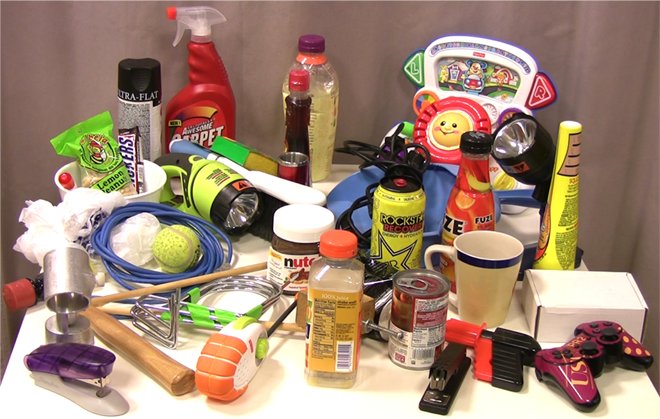
\includegraphics[width=\linewidth]{figs/clutter.png}
	\caption{Robot Operating in Clutter: TODO: Put in a better picture}
	\label{fig:intro}
\end{figure}
%[TODO: Insert picture of experimental setup from simulation]

% With the rapid progress of robotics research, the utility of autonomous robots is no longer restricted to controlled industrial environments. The focus has shifted to high-level interactive tasks in complex environments. The effective execution of such tasks requires the addition of semantic information to the traditional traversability representation of the environment. For example, a household robot needs to be able to detect an object of interest among those scattered on a dining table. For manipulation, it needs to estimate the object's pose accurately.
% 
% One of the central problems in computer vision, object detection and pose estimation, historically has been addressed with the assumption that the position of the sensing device is fixed \cite{Lowe04}, \cite{BelongieMP02}, \cite{FanMN89}. However, occlusions, variations in lighting, and imperfect object models in realistic environments decrease the accuracy of single-view object detectors. 
% 
% Active perception approaches circumvent these issues by utilizing appropriate sensing settings to gain more information about the scene. A large body of research in \textit{sensor management} \cite{Hero11_sensor_management} presents a structured approach to controlling the degrees of freedom in sensor systems and satisfying operational constraints while achieving the task objectives. However, most of the work either assumes  a simplified model for the detection process \cite{spaan08_POMDP, Jenkins10_PhD} or avoids the problem altogether and concentrates on estimating a target's state after its detection \cite{Hero03_sensor_management, sommerlade08_information, Mihaylova03_active_sensing}.
% 
% This paper is a step towards bridging the gap between the research in sensor management and the recent advances in 3D object detection enabled by the advent of low cost RGB-D cameras and open-source point cloud libraries \cite{Rusu_ICRA2011_PCL}. Rather than placing the burden of providing perfect results on a static detector, the sensor can move to increase the confidence in its detection. We consider the following problem. A mobile sensor has access to the models of several objects of interest. Its task is to determine which, if any, of the objects of interest are present on a cluttered table and to estimate their poses. The sensor has to balance the detection accuracy with the time spent observing the objects. The problem can be split into a static detection stage followed by a planning stage to determine a sequence of points of view, which minimize the mistakes made by the observer.
% 
% The rest of the paper is organized as follows. The next section provides an overview of related approaches to active object detection and summarizes our contribution. In section \ref{sec:problem} we draw up hypotheses about the class and orientation of an unknown object and formulate the active detection problem precisely. Section \ref{sec:obj_detect} describes our approach to static detection using a depth camera. In section \ref{sec:obs_model} we discuss the generation of an observation model, which is used in a Bayesian framework to assign a confidence measure on the hypotheses. Section \ref{sec:hyp_test} presents a formalism, which allows testing the hypotheses based on the sensor's observations and selecting a sequence of view-points to balance the sensing time with the decision accuracy. Implementation details are discussed in Section \ref{sec:impl_det}. Finally, in section \ref{sec:experiments} we present simulation results and discuss the validity of our approach.

%\newpage

%\begin{enumerate}
%	\item Why is the problem important? Give motivation and introduction!
%	\item Explain the scenario considered  and the approach to solving the problem
%	\item Talk about other approaches and differentiate the work from them
%	\item Explain the contributions and importance of the work
%\end{enumerate}

%As a result of the latest advances in robotics research, robots are beginning to move away from traditional tightly controlled industrial environments into more complex and dynamic environments. To effectively operate in these environments, the focus of robotic task specification has shifted towards more high-level interactive tasks. For the successful execution of these tasks, the robot requires additional semantic information to be incorporated into the traditional traversibility representations of the environment. For example, a household robot that needs clear a table has to be able to determine if there are any bottles among the objects present on the table. Upon the detection of such objects of interest the robot also needs to estimate the pose accurately enough to manipulate these objects.
%need to detect objects of interest and estimate their location and orientation accurately enough for grasping and manipulation tasks.


%One of the central problems in \textit{computer vision} is object detection and pose estimation. This problem when incorporated into high level task specification also requires the efficient estimation of semantic context with respect to the task. Historically, object detection and pose detection has been addressed with the assumption that the positions of the sensors are fixed ~\cite{Lowe04},~\cite{BelongieMP02} and ~\cite{FanMN89}
%Though there have been a wide variety of techniques developed to address the stationary sensor case, it still remains an open problem as it is consistently plagued by false positives and false negatives. Attempting to develop a perfect object detector for a single viewpoint is an unrealistic task for real world environments as occlusions, variations in lighting and imperfect object models limit the detection capabilities of most algorithms.

%Object recognition is one of the core problems in computer vision, and it is a very extensively investigated topic. Due to appearance variabilities caused for example by non-rigidity, background clutter, differences in viewpoint, orientation, scale or lighting conditions, it is a hard problem.

%Object occlusions, poor lighting or ambiguities of object models limit the detection capabilities of any approach that relies on a single point of view. 


%This paper is a step towards bridging the gap between the research in sensor management while utilizing state of the art techniques in 3D object detection which have gained traction since the advent of low cost RGB-D cameras and the availability of open source libaries for 3D object detection ~\cite{Rusu_ICRA2011_PCL}. Rather than relying entirely on the object detector for perfect estimation, the mobile sensor can execute appropriate actions to improve its detection.
